\subsection{Overall accuracy of Simplified Ikeda method}
\label{se:overall_comparison}
An investigation of how well the implementation of the Simplified Ikeda method (see section \ref{se:simplified_ikeda}) agree with the corresponding result in the roll damping database has been carried out.

Figure \ref{fig:B_e_hat_ikeda_zero} and \ref{fig:B_e_hat_ikeda} show a comparison of the non dimensional equivalent linear damping $\hat{B_e}$
from model tests and the simplified method. Where predicted damping with Simplified Ikeda has been plotted against corresponding test in the roll damping database.  

The test setup in the free roll decay tests differs however from the forced roll motion model tests that Ikeda \cite{ikeda_velocity_1979} used to derive the original method. This is not believed to have any large impact as long as roll damping near the natural frequency is considered. The Ikeda model tests were also conducted with smaller models (2 meters compared to 3-6 meters). But there is a skin friction component $B_F$ to the Ikeda method that should handle this scale effect.

\begin{figure}[H]
    \centering
    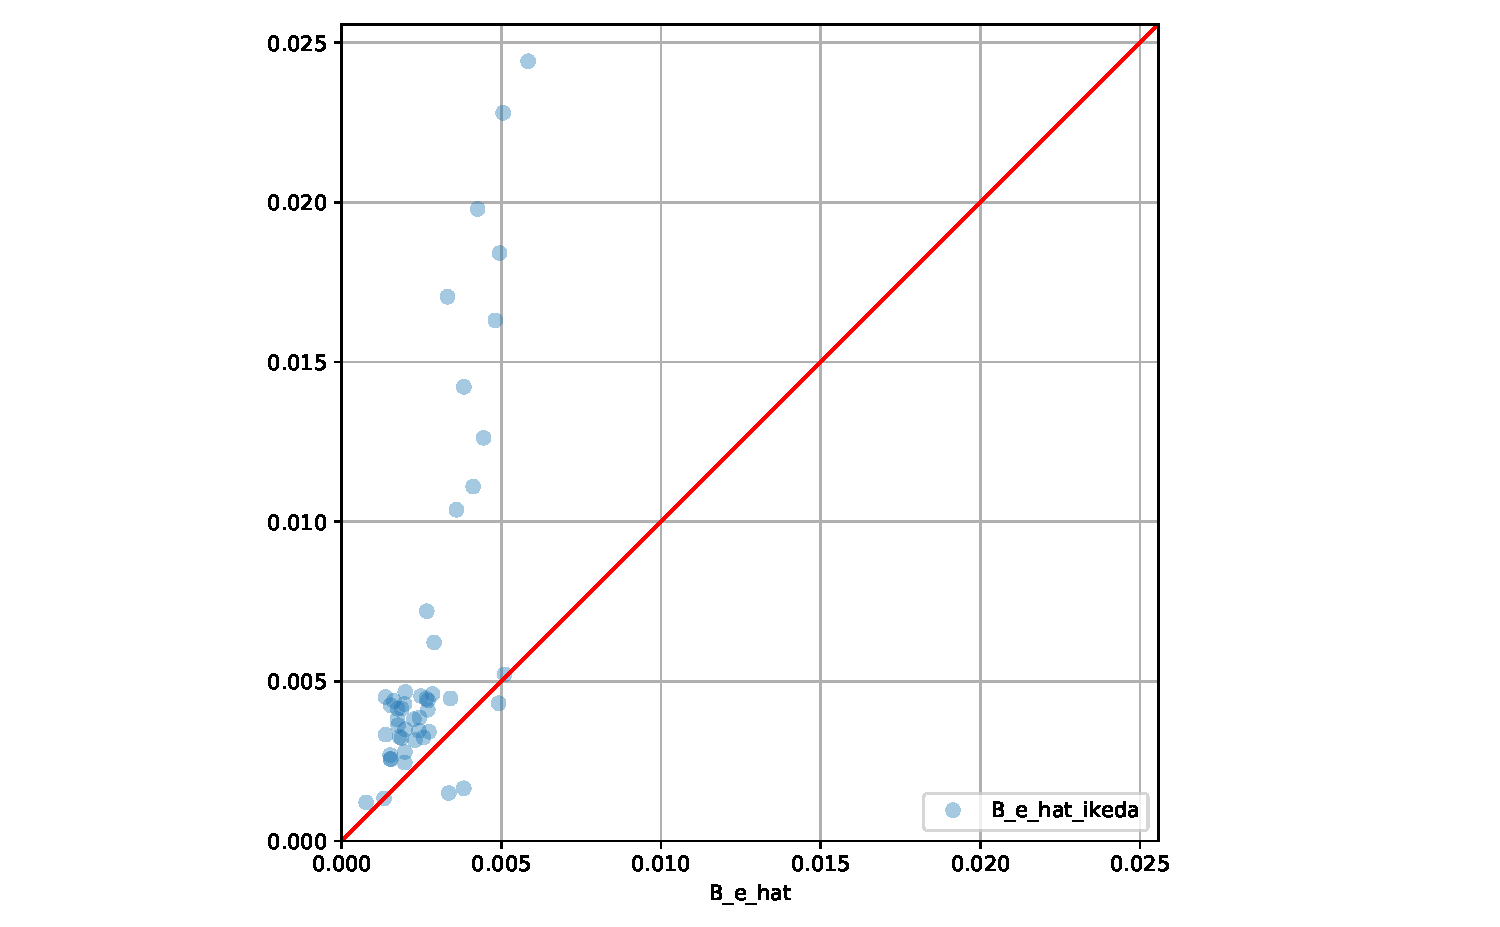
\includegraphics[width=0.9\columnwidth]{figures/B_e_hat_ikeda_zero.pdf}
    \caption{$\hat{B_e}$ comparison at zero speed}
    \label{fig:B_e_hat_ikeda_zero}
\end{figure}

\begin{figure}[H]
    \centering
    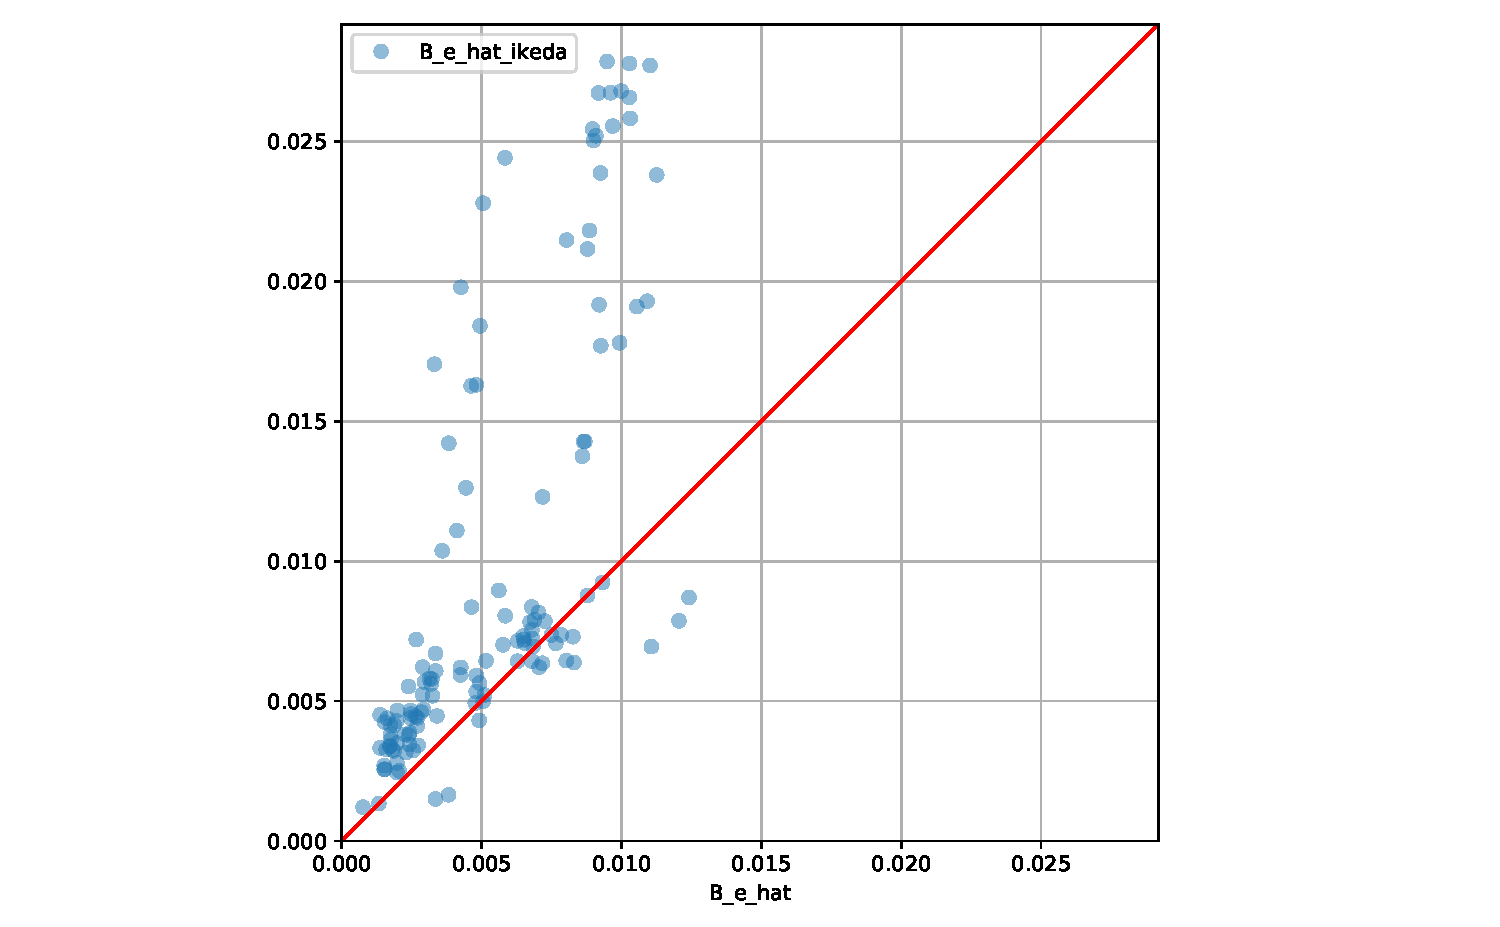
\includegraphics[width=0.9\columnwidth]{figures/B_e_hat_ikeda.pdf}
    \caption{$\hat{B_e}$ comparison at all speeds}
    \label{fig:B_e_hat_ikeda}
\end{figure}

The comparison show poor agreement, both at speed and zero speed. It was discovered that the prediction error was highly depending on the ship draught $T$ which is shown in figure  \ref{fig:B_e_hat_error}.
The figure shows that the error is much larger for $T/L_{pp}<0.034$. Also high frequencies ($\hat{\omega_0} > 0.6$) had higher errors.

\begin{figure}[H]
    \centering
    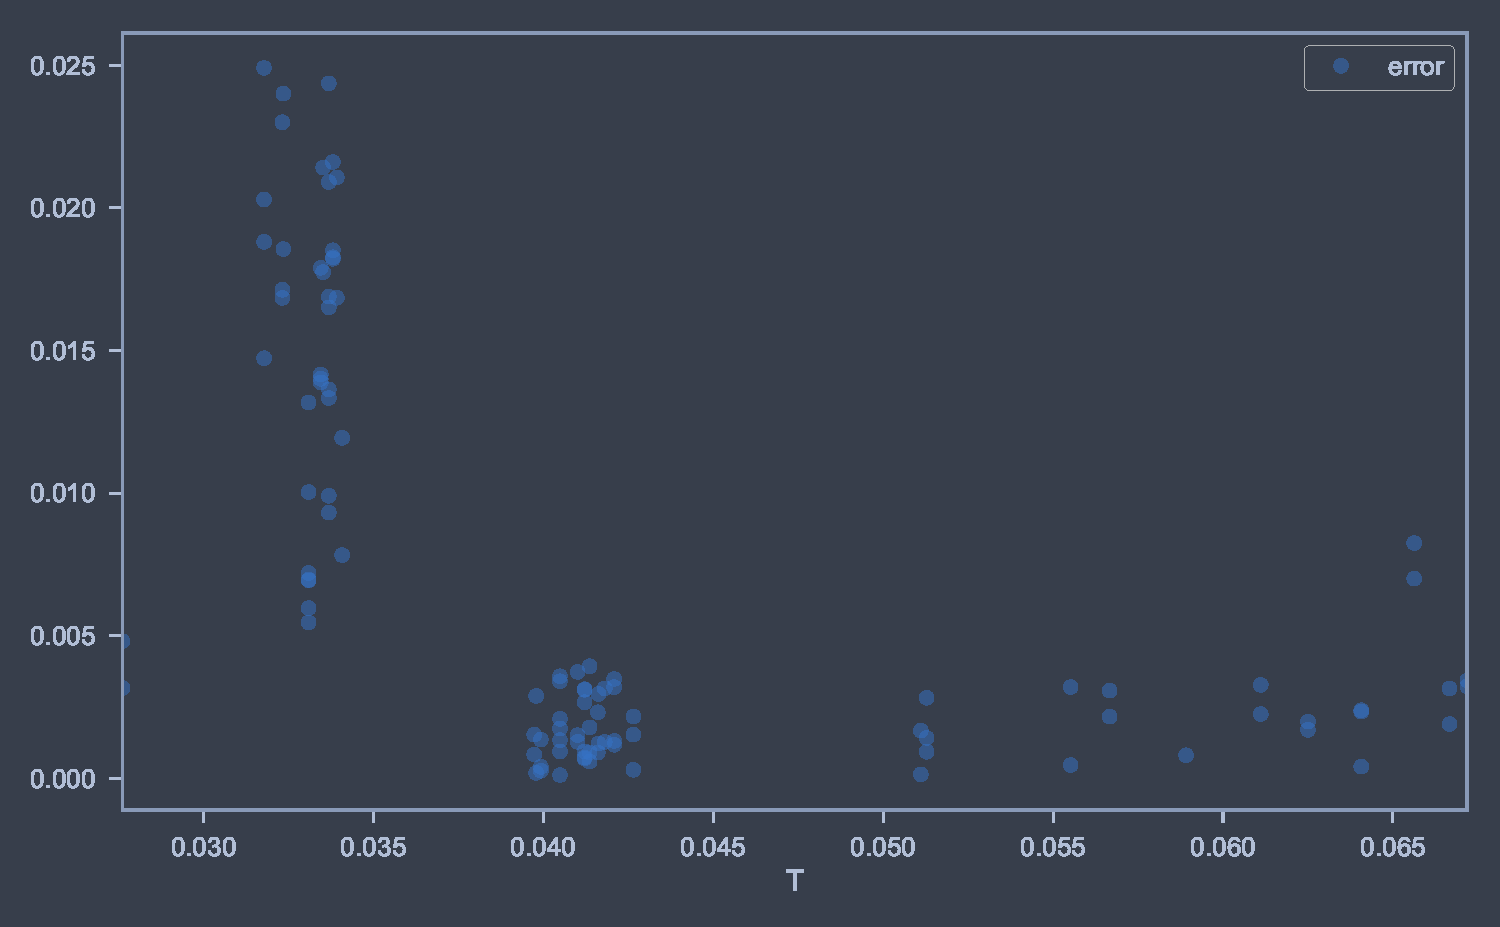
\includegraphics[width=\columnwidth]{figures/B_e_hat_error.pdf}
    \caption{Simplified Ikeda error versus draught}
    \label{fig:B_e_hat_error}
\end{figure}

\begin{figure}[H]
    \centering
    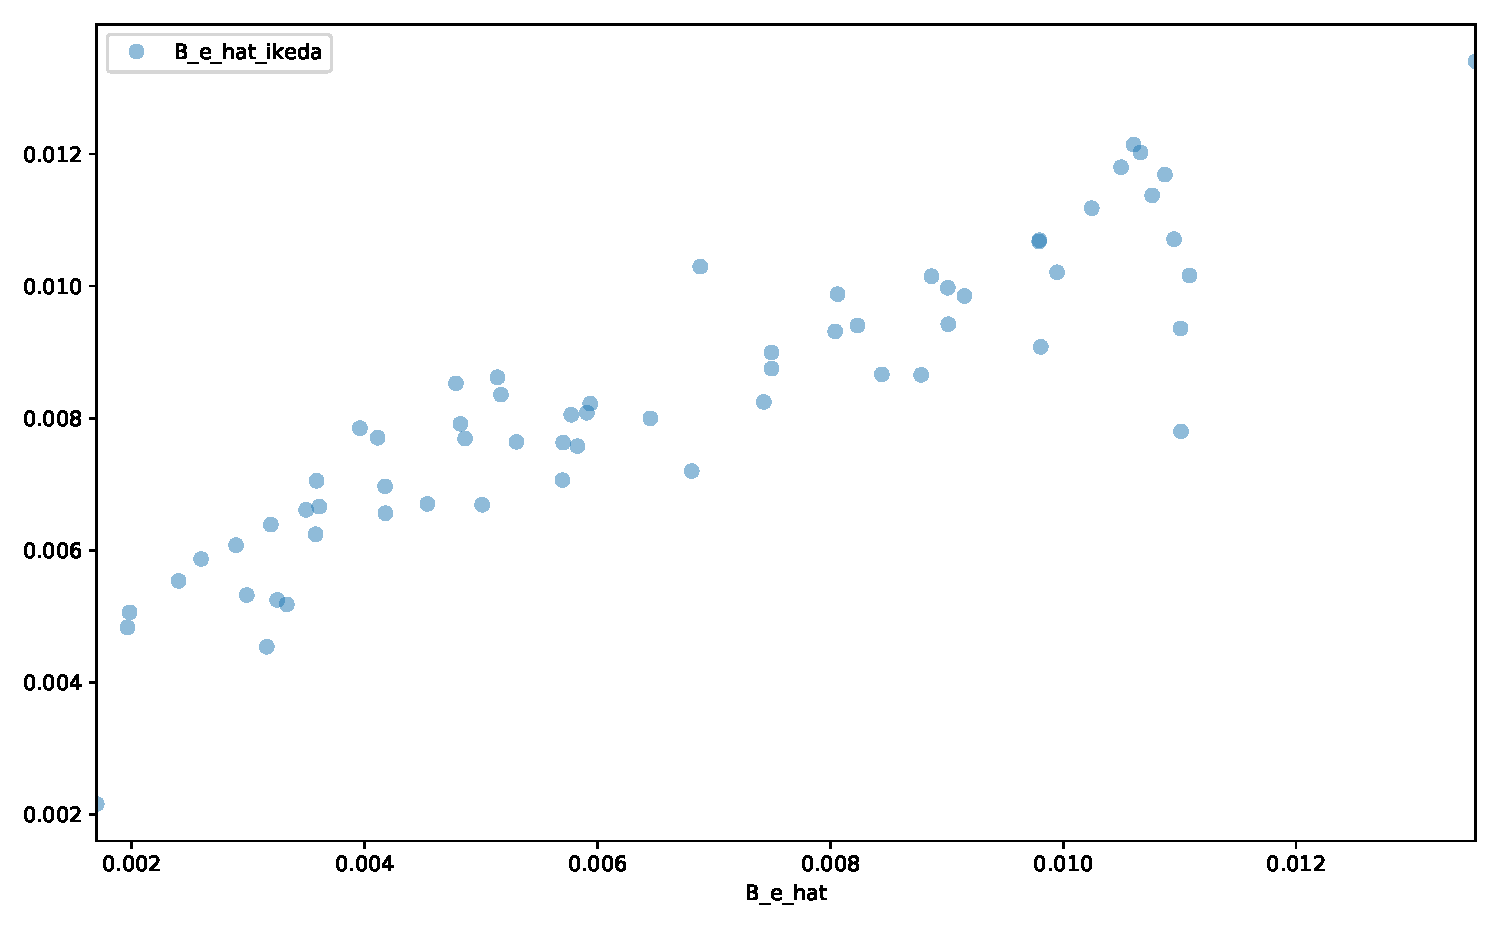
\includegraphics[width=\columnwidth]{figures/B_e_hat_good.pdf}
    \caption{$\hat{B_e}$ comparison with $T/L_{pp}>0.034$}
    \label{fig:B_e_hat_good}
\end{figure}

Figure \ref{fig:B_e_hat_good} shows the comparison for only model tests with $T/L_{pp}>0.034$ and $\hat{\omega_0} < 0.6$.
This confirms the small draft to beam ratio limit of this method as mentioned in \cite{kawahara_simple_2011}. The corresponding $R^2$ score is 0.38.

